\chapter{User Documentation} % User guide
\label{ch:user}

This chapter contains a brief description of the project, a guide on how
to install and run the analyzer, and the way to use it.

\section{Project Description} % Enumerations and lists
This project is a log analyzer working alongside the PipeRT framework
with its profiler. The project aims to analyze the continuous stream of
data coming from the PipeRT's profiler, in a server-client relationship.

The analyzer was built using \textit{Python} regarding the back-ends and \textit{Javascript} regarding the frontend,
it provides various checkers to investigate the sanity of the pipeline created 
by the PipeRT's user, graphs associated with the measurements, and visualization
of the pipeline and how the channels are structured.

The analyzer in itself was built to be an analyzing framework where
extensibility was the key and will be in the design decisions, so as a result,
it is relatively easy to add new features and already prepared to be extended
by new checkers and measurements.


\section{Installation Guide}\label{sec:installiation_guide}
PipeRT is currently supporting Linux only, but soon,
it will support Windows as well. That said, the steps to install
the analyzer are the same in both operating systems.

To download PipeRT, please clone the repository from \url{https://github.com/gerazo/pipert}.

The \textbf{\url{log_analyzer}} folder inside the PipeRT project folder
is where all of the Installation steps will take place.

Python 3.9 should be installed on the operating system. All the
requirements can be installed by typing the following command in
the terminal or the command prompt.
\newline
\begin{lstlisting}[language=bash, caption={Install requirements},captionpos=b]
	$ pip install requirements.txt
\end{lstlisting}

It is also recommended to create a python virtual environment
before installing the requirements, in order to have a separate
environment for the analyzer. The commands to create and run the environment
are:
\newline
\begin{lstlisting}[language=bash, label={code:venv}, caption={Create and run virtual environment},captionpos=b]
	$ python3 -m venv venv	
	$ source venv/bin/activate
\end{lstlisting}


\subsection{Running} % Framing figures
In order to run the analyzer make sure to be inside the
\textbf{\url{log_analyzer}} folder and type the following
command:
\newline
\begin{lstlisting}[language=bash, caption={Start application},captionpos=b]
	$ python start.py
\end{lstlisting}

This will start the application, so once you type \url{127.0.0.1:5000}
in the browser (Firefox recommended). You will be able to see the following:
\newline
\begin{figure}[H]
	\centering
	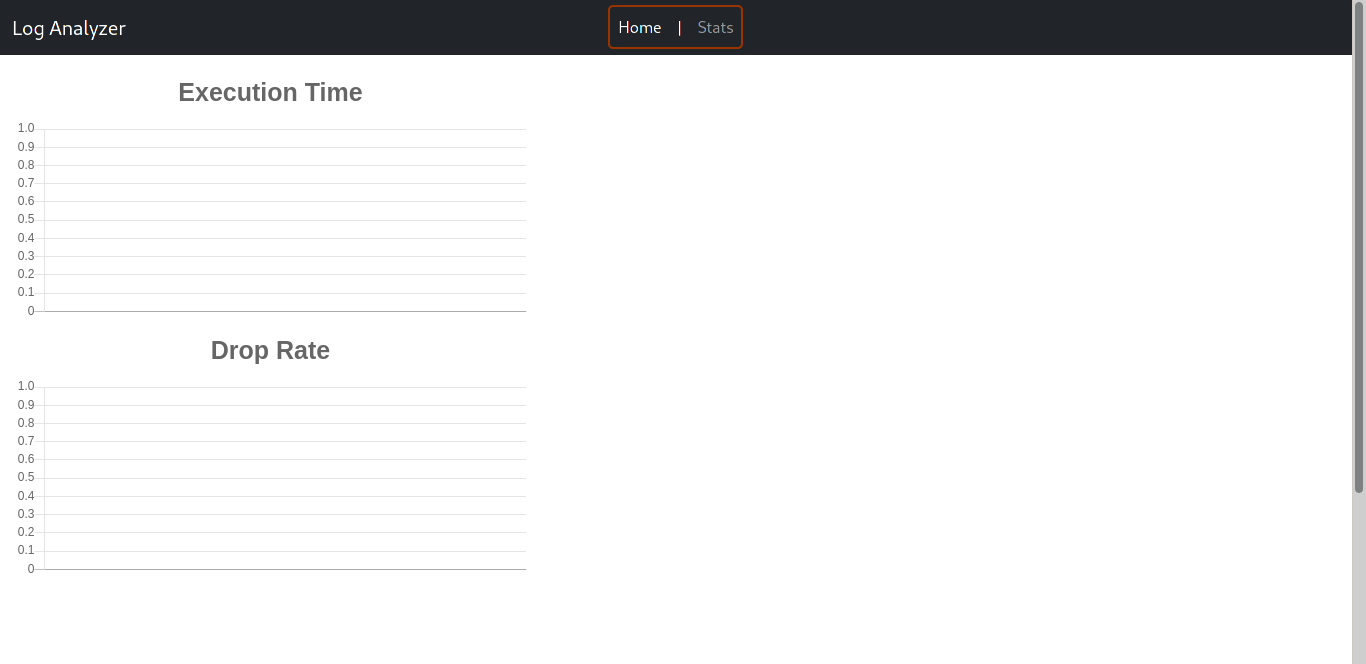
\includegraphics[width=0.9\textwidth,height=175px]{images/start.png}
	\caption{Start of the application}
	\label{fig:empty_page}
\end{figure}

\section{Client-Server Configuration} % Tables
To establish a connection between the profiler (Client)
and the log analyzer (server), there should be modifications in both
sides.

\subsection{Client Side} \label{sec:server_side_config}

The profiler is the utility for monitoring the DSP pipeline and sending logs,
it has 3 arguments:
\begin{itemize}
	\item \textbf{\url{destination_uri}}, which describes the destination and the used protocol, udp and file 
	are the protocol options in the profiler currently.
	\item \textbf{\url{aggregation_time_msec}} which is the time in milliseconds to wait 
	before gathering monitoring data again, so it determines how often aggregated
	log data is sent to the log processor, if not given that means not to collect
	periodically.
	\item \textbf{\url{buffer_size}}, it controls the size
	of buffer which is filled to be sent at once, the default value depends on the
	protocol chosen.
\end{itemize} 

To establish a connection with the analyzer, the udp protocol
is the one to choose, the IP and socket are based on the user
preference (port 5000 can not be chosen because that is the port
for the analyzer interface).

Adding the profiler to the scheduler is the last step to configure
the client-side, and the following example shows how to add the profiler.
\newline
\begin{lstlisting}[language=c++, caption={Adding the profiler},captionpos=b]
	pipert::Scheduler sch(0, pipert::Profiler("udp:127.0.0.1:8000"));
\end{lstlisting}

\subsection{Server Side}\label{client_side}
On the server-side, the same port number that has been provided to the profiler
should be added in the \textbf{config.json} inside the \textbf{\url{log_analyzer}} folder. same for
the IP as well.
\newline
\begin{lstlisting}[language=bash, caption={connection configuration},captionpos=b]
{
    "port": 8000,
    "ip": "127.0.0.1"
}
\end{lstlisting}

An important note: The log analyzer does not show any effect on the page until the end of a packet cycle
\ref{sec:g_config}, so, the web page will be the same as \ref{fig:empty_page} 
until the completion of the first cycle.

\section{Analyzer Configuration}
The log analyzer is made to check the sanity and analyze various
applications and systems, so having a configuration was essential.

The configuration is a \textit{JSON} (JavaScript Object Notation) file,
the choice of the format to be JSON was due to its
lightweight, well-known among developers, and simplicity. 
The config.json configuration file consists of 3 main parts, 
general, measurements' and checkers' configurations. Let's enumerate them.
\newline
\begin{lstlisting}[language=bash, caption={Sample configuration},captionpos=b, label={lst:sample_confing}]
	{
		"PORT": "8000",
		"IP": "127.0.0.1",
		"PACKET_CYCLE_THRESHOLD": 1000,
		"pipeline_measurements": [
			{
				"name": "pipeline_measurement_1",
				"enabled": true,
				"key": "Pipeline Measurement 1"
			}
		],
		"channel_measurements": [
			{
				"name": "channel_measurent_1",
				"enabled": true,
				"key": "Channel Measurement 1"
			}
		],
		"checkers": [
			{
				"name": "checker_1",
				"enabled": true,
				"measure_key": "Channel Measurement 1",
				"parameters": {
					"THRESHOLD": 20
				}
			}
		]
	}
\end{lstlisting}

\subsection{General Configurations} \label{sec:g_config}
Consist of 3 configurations, \textbf{PORT}, \textbf{IP}, 
and \textbf{\url{PACKET_CYCLE_THRESHOLD}}. The first two were discussed in \ref{client_side}.

The \textbf{\url{PACKET_CYCLE_THRESHOLD}} is an integer value that describes
how many packets should the analyzer receive before running the checkers once
and these packets' events will be stored in the channels and when the cycle
finishes (when the number of packets received is equal to \textbf{\url{PACKET_CYCLE_THRESHOLD}}), these
events will be deleted from the channels and a new packets cycle starts.
\newline
\begin{figure}[H]
	\centering
	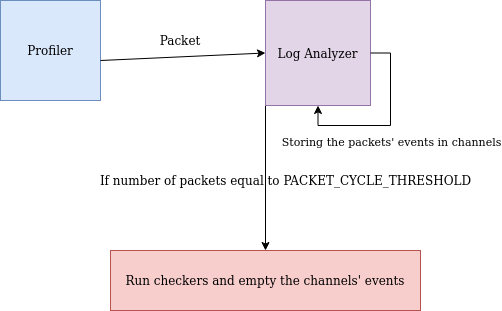
\includegraphics[width=0.9\textwidth,height=200px]{images/packets_cycle.png}
	\caption{Packet cycle}
	\label{fig:packets_cycle}
\end{figure}

\subsection{Measurements' Configurations}
These configurations are split into two categories, the pipeline's measurement, and
the channel's measurements. Despite their difference from the measuring point of view
as discussed in \ref{sec:measures}, they do share the same configuration's style. (\ref{lst:sample_confing})

Both of the two measurements are a list of dictionaries, where each dictionary
represents a measurement, and each measurement has three key-value pairs,
\textbf{name}, \textbf{enabled}
to turn the measurement on or off, and \textbf{key} this will be the shown
text for the measurement and will also help to connect the measurement to 
a specific checker if needed.

\subsection{Checkers' Configurations}
The checkers' configuration is a
list of dictionaries where each dictionary is a checker's configuration. Each configuration
contains the checker's name in the \textbf{name} field, whether it should work or not in
the \textbf{enabled} field, \textbf{measure\_key} to specify the measurement
for that checker if needed, and a \textbf{parameters} field where the parameter
of the checker can be created or changed.

The \textbf{name} field should be the same name as the file of the checker or the measurement
without the extension (.py). And that is how the dynamic importing module in 
the project will be able to import the checker with its configuration \ref{sec:config_utils}.

The \textbf{enabled} field is a boolean field to turn on or off the checker.

The \textbf{measure\_key} field is a string to connect the checker with
its corresponding measurement.

The \textbf{parameters} field is a dictionary with as many keys as the checker's
parameters. These values can be changed based on the DSP application using the
analyzer, and it is the user's responsibility to assign the appropriate values.

\section{Measurements} \label{sec:measures}
The backbone of the log analyzer is the measurements, and that is the reason for implementing
various of them, given these varieties of measurements, it is expected to
help to check the sanity of the pipeline and spotting the bottlenecks for the user. They
are also essential for most of the checkers (more about it in \ref{sec:checkers}).

They consist of two categories, \textbf{channel's} and \textbf{pipeline's} measurements. All the
measurements run once per packet cycle and the graphs resulted should be drawn every ten cycles,
as can be seen from figure \ref{fig:measurement_graph}. The following pages contain a detailed description
of the categories and their measurements.

The profiler and its events are described in detail at \ref{sec:profiler}, the measurements
use these events as an input to produce results.
\newline
\begin{figure}[H]
	\centering
	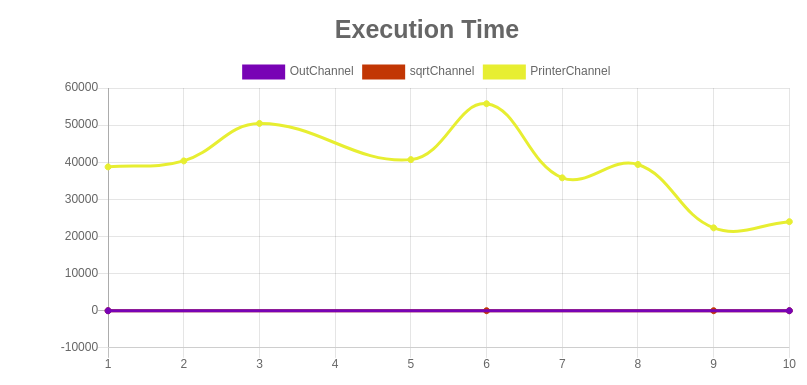
\includegraphics[width=0.9\textwidth,height=200px]{images/basic_graph.png}
	\caption{Measurement's graph}
	\label{fig:measurement_graph}
\end{figure}

\subsection{Channel's Measurements}
The measurements in this section focus on the channels and their attributes. They are seven implemented
measurements, and the details of them will be explained below.

\subsubsection{Drop Rate Measurement}
Calculating the number of dropped events over the number of executed events. In case of no executed events,
the result will be \textbf{1}, if no dropped events, it will return \textbf{-1}, and if both events are missing
\textbf{-1} will be the output of the calculation.

\subsubsection{Drop Ratio Measurement}
Calculating the number of dropped events over the number of read events. In case of no read events,
the result will be \textbf{1}, if no dropped events, it will return \textbf{-1}, and if both events are missing
\textbf{-1} will be the output of the calculation.
 
\subsubsection{Execution Time Measurement}
This measurement is responsible of calculating the average of the execution time by dividing the sum
of the execution time events' average over the number of the execution time. In case the is no execution
time events, it will output \textbf{-1}.

\subsubsection{Fill Time Measurement}
Its responsibility is calculating the average of the fill time by dividing the sum
of the fill time events' average over the number of the fill time. In case the is no fill
time events, it will output \textbf{0}.

\subsubsection{Time To Buffer Average Measurement} \label{sec:time_to_buffer_average}
It calculates the average value of the buffering time. The buffering time is the time
packets spend from the end of the execution in the previous channel  
till they are buffered in the current channel.

\subsubsection{Read Time Measurement}
Measure the average read time of the packets, if there are no read events, it will return zero.

\subsubsection{Packet Life Time Measurement}
Calculates the ratio of the time the packets spent in all the channels to the time spent in a channel. 
The time packets spend is the average sum of fill time, read time, execution time, packet pushed, 
and packet retrieved events.

\subsection{Pipeline's Measurements}
The measurements in this category use all of the gathered information from all the channels in the pipeline.
There is one implement measurement, and it is the \textbf{Total Execution Time Ratio Measurement},
it calculates the ratio between the execution time events and the 
total time the packets spent in the pipeline, in other words, it calculates the ratio of pipeline thrust time to
the total execution time of all channels.

\section{Checkers}\label{sec:checkers}
Checkers results flags and measurements of different aspects of the channel and pipeline. All 
the enabled checkers run for all the channels in the pipeline and in case the check passes, it will appear
in the webpage as in \ref{fig:passed_checker}, on the other hand, figure \ref{fig:failed_checker} shows 
the representation of a failed check in the current packets cycle.
\newline
\begin{figure}[H]
	\centering
	
\includegraphics[width=0.9\textwidth,height=50px]{images/passed_checker.png}
	\caption{Passed checker}
	\label{fig:passed_checker}
\end{figure}

\begin{figure}[H]
	\centering
	
\includegraphics[width=0.9\textwidth,height=50px]{images/failed_checker.png}
	\caption{Failed checker}
	\label{fig:failed_checker}
\end{figure}
The checkers are stateless, so no information from the previous cycles is saved. Each checker has a name, 
can have a configuration, and a description of what does it check. We are going to enumerate these information
in the following pages.

\subsection{Frozen Checker}
The checker name on the webpage is \textbf{\url{FROZEN}}, it checks if a channel received one or more events in the last packets cycle, 
if it did not receive any, the check fails for this cycle.

\subsection{Drop Rate Checker}
The name on the webpage is \textbf{\url{HIGH_DROP_RATE}}, it Calculates the drop rate of 
a channel (see \ref{}), and passes if and only if the rate is bigger than the configured threshold value. The
configuration consists of one key-value pair, \textbf{\url{DROP_RATE_THRESHOLD}} is the key, and the already configured
value is \textbf{0.5}.

\subsection{Drop Ratio Checker}
The name on the front-end is \textbf{\url{HIGH_DROP_RATIO}}, it is responsible for calculating the drop ratio
(see \ref{}), and if the calculated value exceeds the threshold configured then the check fails. The 
\textbf{\url{DROP_RATIO_THRESHOLD}} is the only configuration and \textbf{0.75} is the default value.

\subsection{Execution Time Checker}
\textbf{\url{HIGH_EXECUTION_TIME}} is the name shown on the page, it checks whether the execution time of a channel
did surpass the configured threshold. The calculation of the execution time can be found at \ref{}. \textbf{0.75}
is the default value for the only configuration \textbf{\url{EXECUTION_TIME_THRESHOLD}}.

\subsection{Read Time Checker}
Very Similar to the \textbf{Execution Time Checker}, but checking for the reading time. The configuration
consists of one key-value pair, which is the \textbf{\url{CHANNEL_READ_THRESHOLD}} and the default value is 
\textbf{20}. The name on the page is \textbf{\url{HIGH_READ_TIME}}. (see \ref{} for the measurement details)

\subsection{Fill Time Checker}
Having the same methodology for checking as the \textbf{Execution Time Checker} and the \textbf{Read Time Checker}.
Its configuration contains only one key-value pair to set the threshold of the filling time of a channel.
\textbf{\url{CHANNEL_FILL_THRESHOLD}} is the configuration's name, and the default value is \textbf{20}. The checker page's
name is \textbf{\url{HIGH_FILL_TIME}}.

\subsection{Time To Buffer Average Checker}
It uses the \textbf{Time To Buffer Average Measurement} (\ref{sec:time_to_buffer_average}) and checks
for the channels if the measurement for them exceeds the configured value if it exceeds the checker
fails.

\section{Graphical User Interface}\label{sec:GUI}
The analyzer interface is a webpage containing two pages, \textbf{Home} and \textbf{Measurements}. In this
section, I will describe the components of each page and the features provided.

The navigation bar (figure \ref{fig:nav_bar}) is shared between the two pages and controls navigating
between the two of them. To load the \textbf{Home} page, you can click on either the \textit{Home} or
\textit{LogAnalyzer}. In case of \textbf{Measurements}, clicking on \textit{Measurements} will load it.
\newline
\begin{figure}[H]
	\centering
	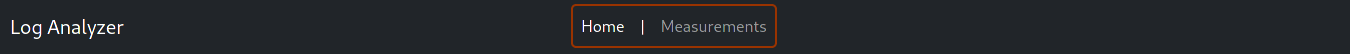
\includegraphics[width=1.1\textwidth,height=40px]{images/nav_bar.png}
	\caption{The navigation bar}
	\label{fig:nav_bar}
\end{figure}

\subsection{Home Page}
The home page should give a brief description of the pipeline's status through its components. It consists
of checkers for channels (\ref{fig:checkers_home_page}), measurements section (\ref{fig:measures_home_page}), 
and pipeline visualization (\ref{fig:pipeline_viz_home_page}).

As mentioned before, before completing the first packet cycle, the home page will look as in figure \ref{fig:empty_page}.
Once the profiler is sending regularly, you can expect to have the home page similar to figure \ref{fig:home_page_running_state}.

Each channel has a corresponding color which is used through the different components in order to ease the
distinguishment and to have a visual identity for each of them.
\newline
\begin{figure}[H]
	\centering
	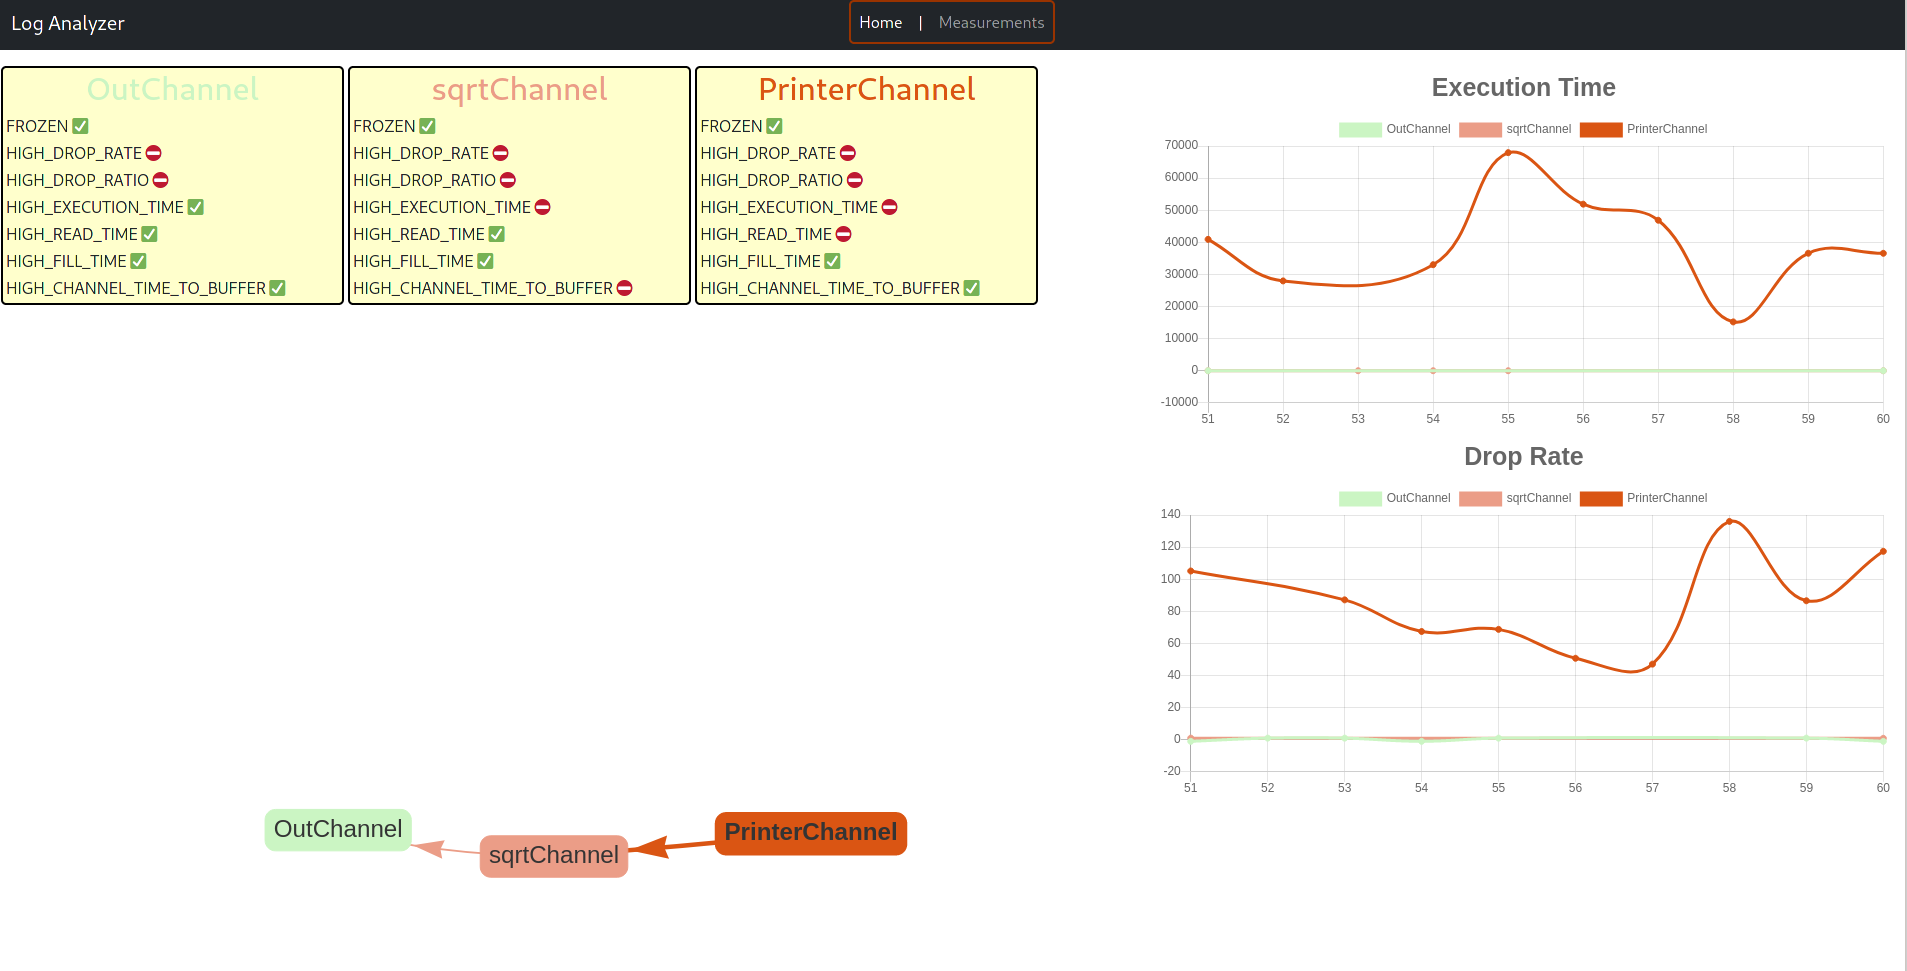
\includegraphics[width=1.0\textwidth,height=300px]{images/home_page_in_running_state.png}
	\caption{Home page in running state}
	\label{fig:home_page_running_state}
\end{figure}

\subsubsection{Channels' Checkers}
They are located in the top left of the home page (\ref{fig:home_page_running_state}), 
each channel is represented as a box where the name
of the channel is at the top of it and the checkers and their status come after. 
\newline
\begin{figure}[H]
	\centering
	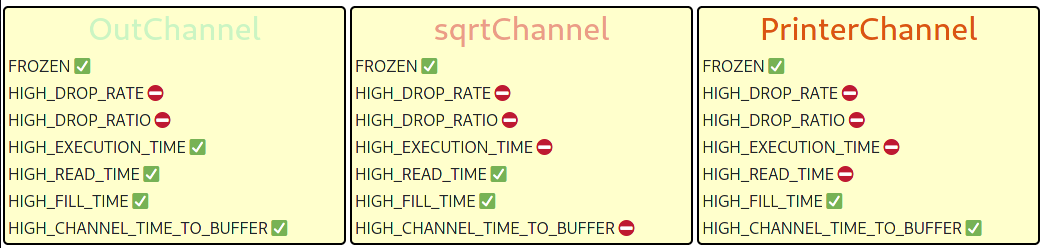
\includegraphics[width=0.9\textwidth,height=200px]{images/checkers_home_page.png}
	\caption{Checkers in the home page}
	\label{fig:checkers_home_page}
\end{figure}

\subsubsection{Measurements}\label{sec:measuremets_home}
They can be found in the top right of the home page (\ref{fig:home_page_running_state}). They are
two measurements on the page, \textbf{execution Time} and \textbf{drop rate}, these two measurements
were chosen because of their capabilities of reflecting important aspects of the channels.
\newline
\begin{figure}[H]
	\centering
	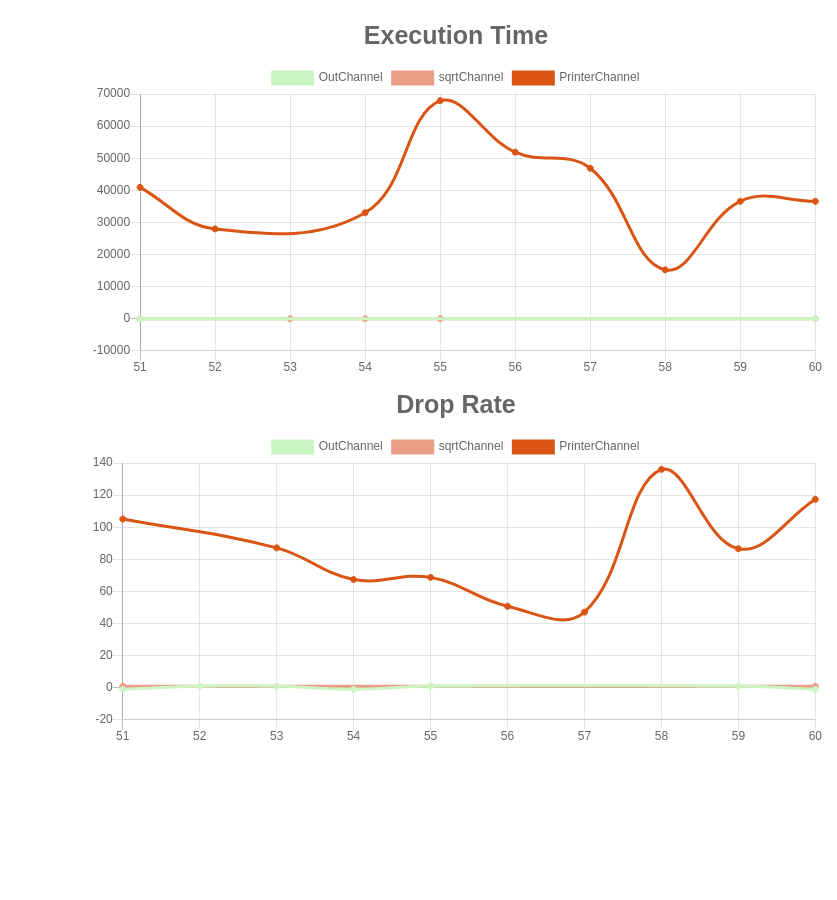
\includegraphics[width=0.9\textwidth,height=300px]{images/measures_home_page.png}
	\caption{Measurements in the home page}
	\label{fig:measures_home_page}
\end{figure}

As shown in figure \ref{fig:measurement_graph}, the name of the measurement is at the top, and the channels'
names and colors following come after, and then the graph itself. Each channel corresponds to the color
on the left of its name.

To be able to see the exact axis of a certain point of the graph, you can hover with the mouse, 
and the result will be as in figure \ref{fig:hover_graph}. The name of the channel and its color
will also be included. 
\newline
\begin{figure}[H]
	\centering
	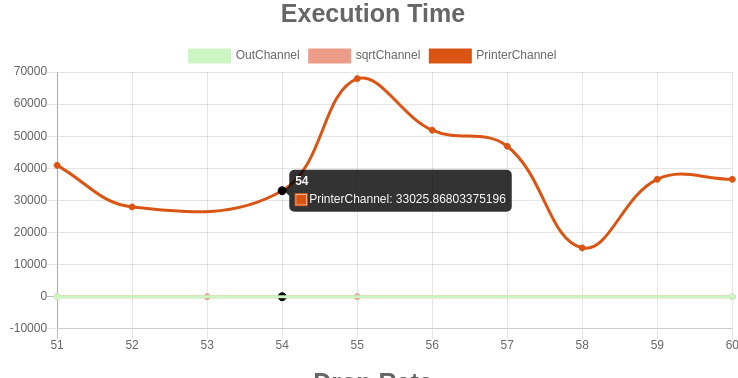
\includegraphics[width=0.9\textwidth,height=150px]{images/hover_graph.png}
	\caption{Hovering a point in a graph}
	\label{fig:hover_graph}
\end{figure}

In many cases, some channels can be unseen because of other channels' high y-axis value. If you want
to hide the channel line graph, you can click on the channel's name or color, and there will be 
a horizontal line on the clicked channel's name to indicate that its measurements is not shown
in the graph. Figure 
\ref{fig:remving_channel_graph} shows the effect of this action.
\newline
\begin{figure}[H]
	\centering
	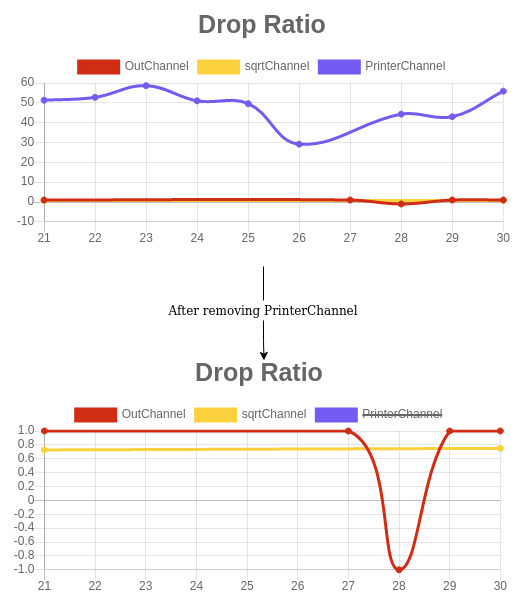
\includegraphics[width=0.9\textwidth,height=300px]{images/removnig_channel_graph.jpg}
	\caption{Graph after removing a channel}
	\label{fig:removing_channel_graph}
\end{figure}

\subsubsection{Pipeline Visualization}\label{sec:pipeline_vis}
It is located at the bottom of the home page. Each box contains the name of a channel, and the box's color is the
channel's color, and the arrows between these boxes represent the connection between the channels in the
actual pipeline created by the user.
\newline
\begin{figure}[H]
	\centering
	
\includegraphics[width=0.9\textwidth,height=150px]{images/pipeline_viz.png}
	\caption{Pipeline's visualization in the home page}
	\label{fig:pipeline_viz_home_page}
\end{figure}

You can change the position of the pipeline visualization by clicking anywhere in the bottom half of the page
beside the channels' boxes themselves and dragging the visualization around. It is also possible to change the 
shape of the visualization or rearrange it by clicking any of the channels' boxes and dragging.
\newline
\begin{figure}[H]
	\centering
	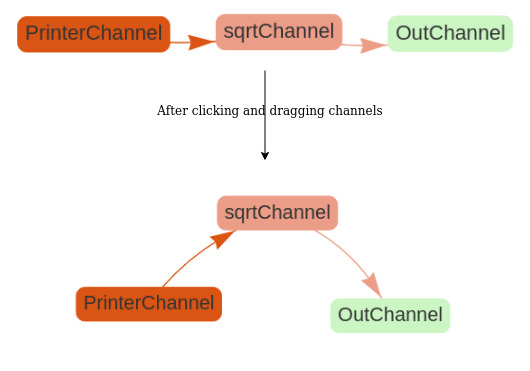
\includegraphics[width=0.9\textwidth,height=250px]{images/moving_viz_graph.jpg}
	\caption{Rearranging the pipeline visualization}
	\label{fig:remving_channel_graph}
\end{figure}

\subsection{Measurements Page}
The page contains all the measurements explained in \ref{sec:measures}, it is divided into \textbf{channels'} and
\textbf{pipeline's} measurements as in figure \ref{fig:measures_empty} and \ref{fig:measures_running_state}. The
channels' measurements come before the pipeline's measurements.

The graphs represent 10 packet cycles of their measurements. Each channel has the same color through all the
various graphs to easily distinguish between each other same as in the \textbf{Home} page.
\newline
\begin{figure}[H]
	\centering
	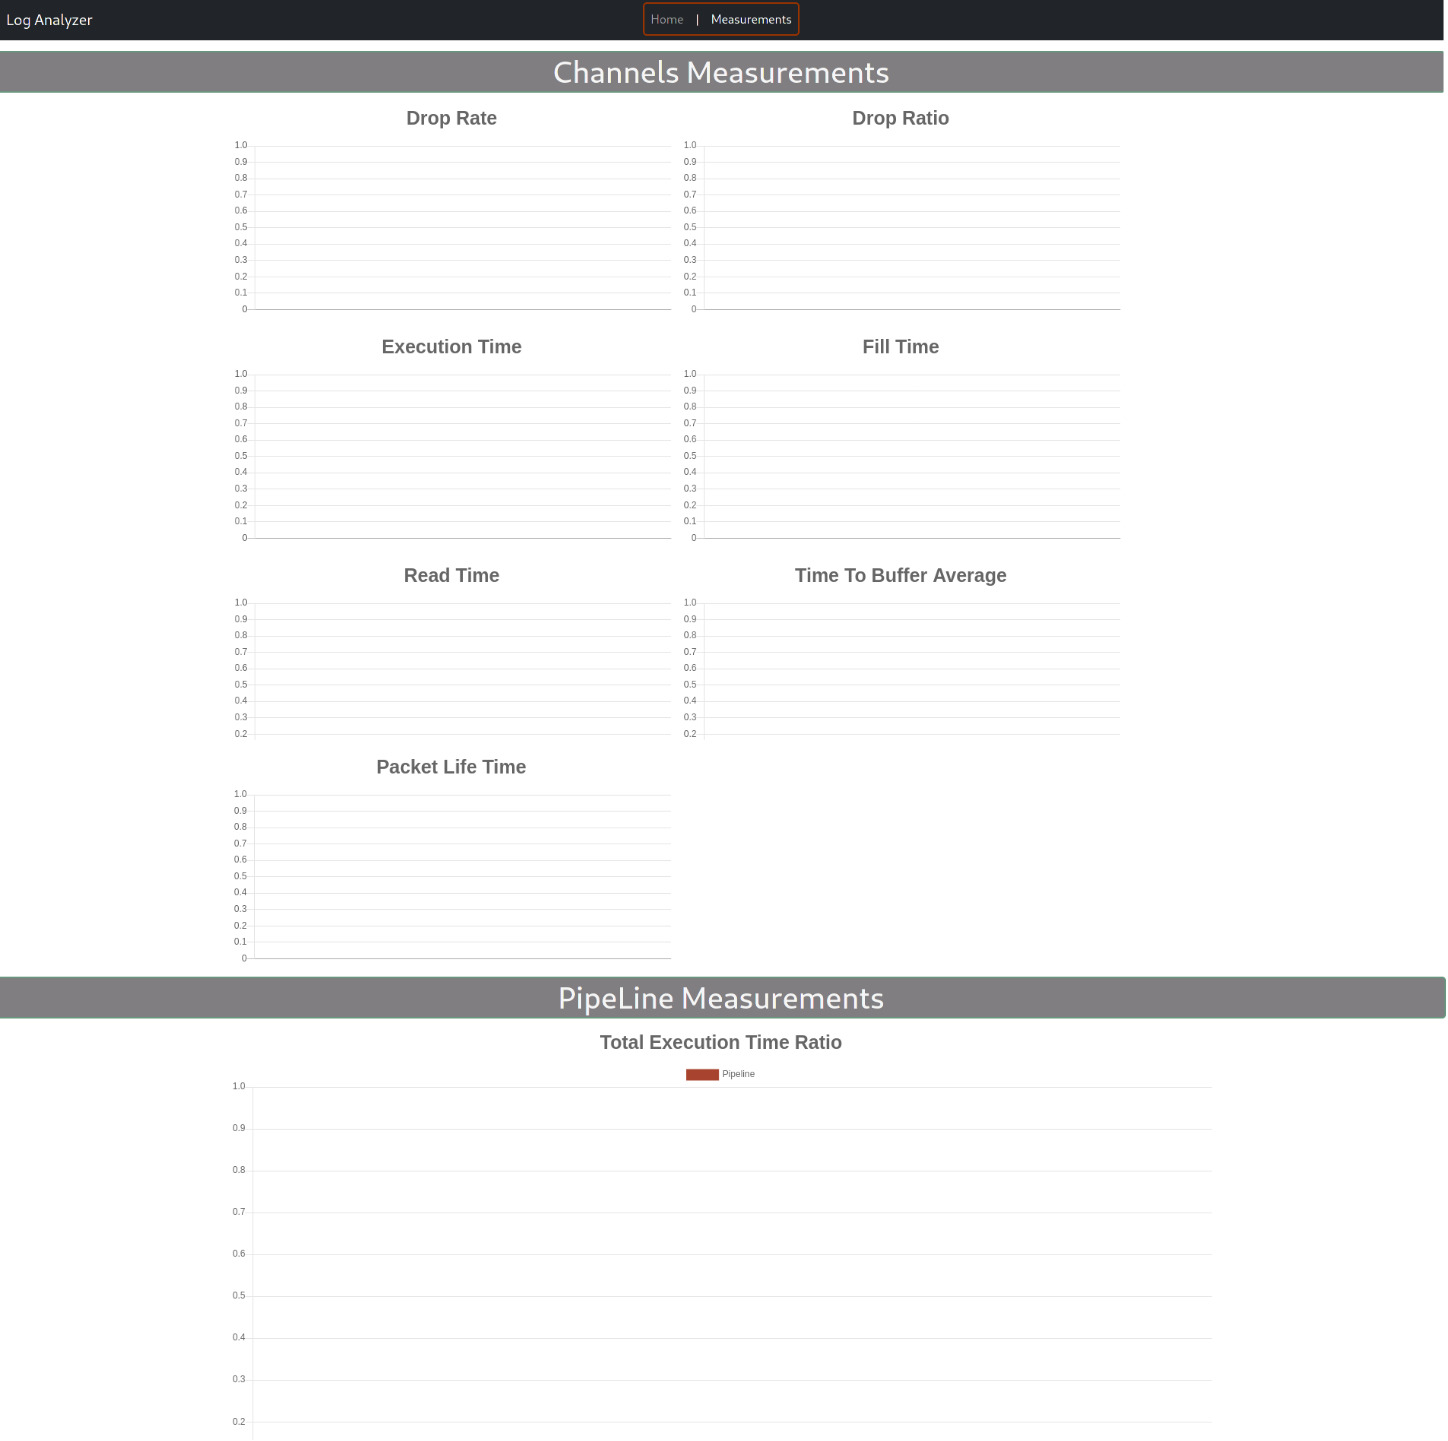
\includegraphics[width=0.9\textwidth,height=350px]{images/measures_empty.jpg}
	\caption{Measurements page in empty state}
	\label{fig:measures_empty}
\end{figure}

All the features that were in the measurements section of the \textit{Home} page (\ref{measuremets_home})
are extended to this page as well, including removing one or more channels from the graph and
seeing the exact coordinate of a point.
\begin{figure}[H]
	\centering
	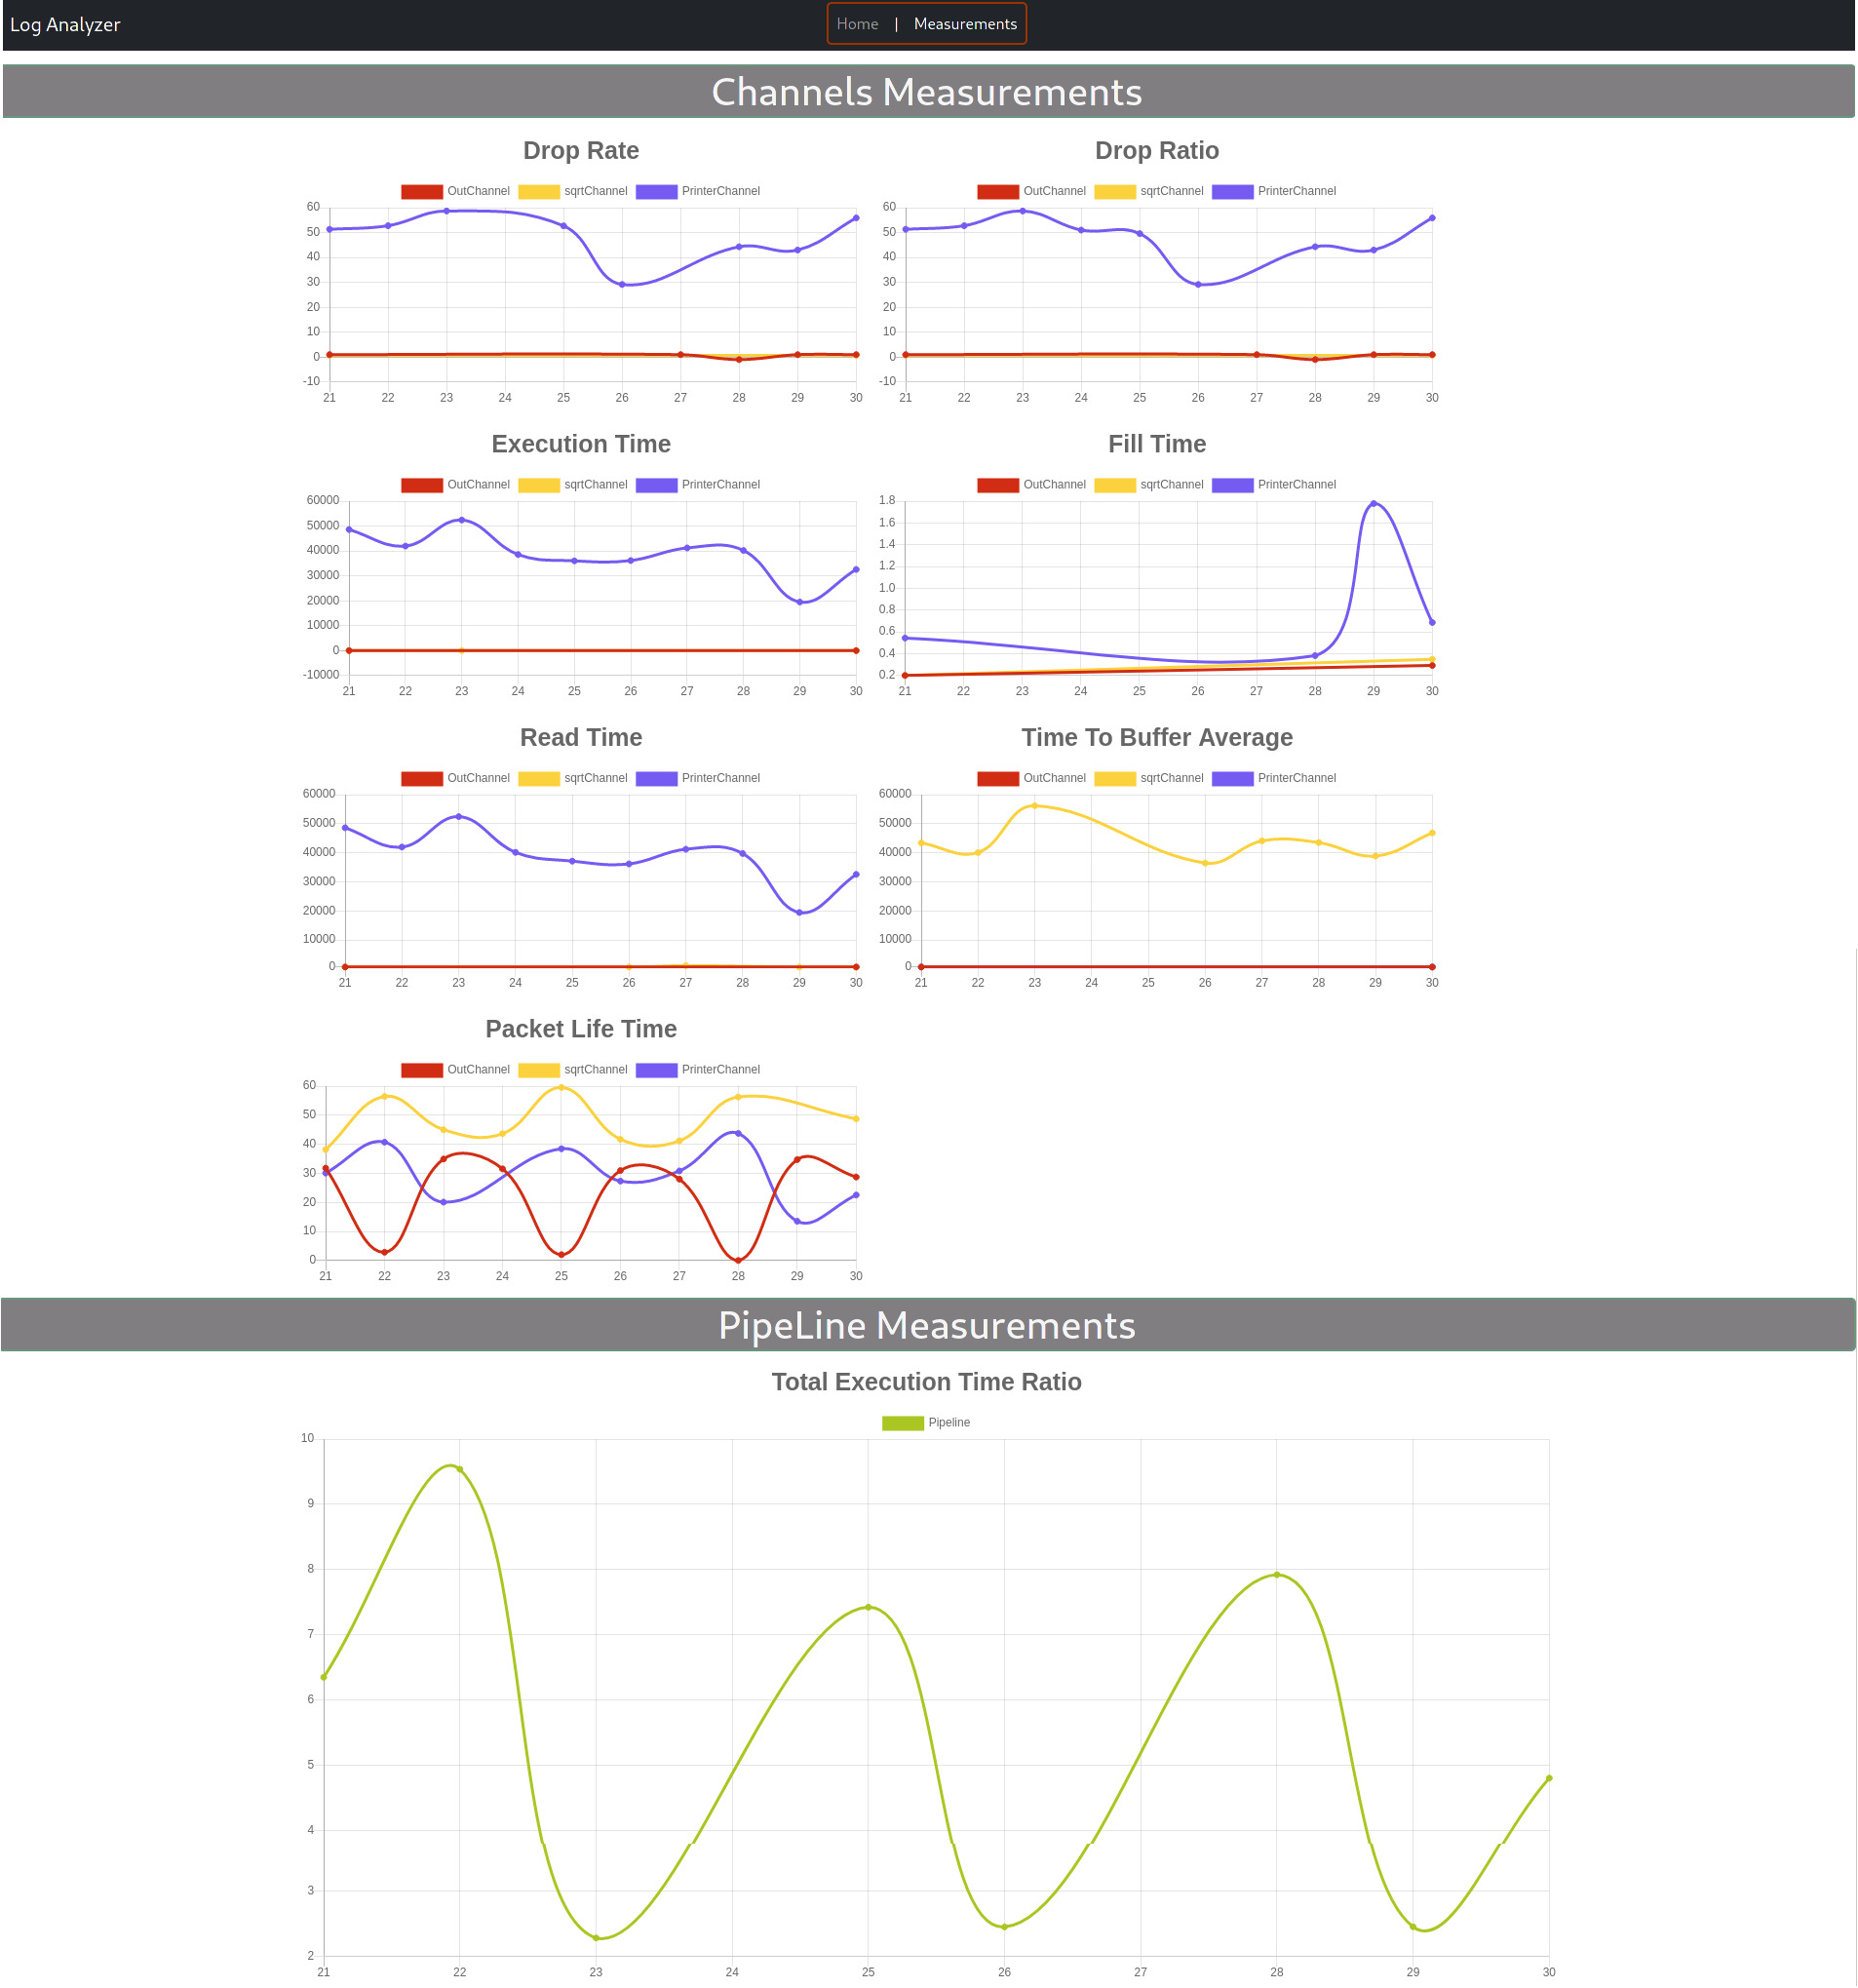
\includegraphics[width=0.9\textwidth,height=350px]{images/measures_running_state.jpg}
	\caption{Measurements page in running state}
	\label{fig:measures_running_state}
\end{figure}